\chapter{Diseño} \label{chap:diseno}
El objetivo de este apartado será explicar el diseño por el que se ha optado tanto físico como lógico y los motivos que han hecho que tomemos esas decisiones. 

\section{Diseño físico del entorno}

Para el dimensionado del entorno físico, se ha tenido en primer lugar en cuenta el objetivo del proyecto. Dado que la motivación del mismo es crear una infraestructura en la que podríamos implementar cualquier servicio y dotarla de mecanismos de orquestación de funciones de red que proporcionen escalabilidad y redundancia para asegurar alta disponibilidad, en principio se pensó el instalar cuatro máquinas distintas: dos en una localización geográfica y otras dos en otra diferente. En cada una de las localizaciones tendríamos un servidor dedicado con los servicios de autenticación (Keystone) y dashboard (Horizon), que compartirían los datos de todos los usuarios y proyectos disponibles, y en los otros dos el resto de servicios de OpenStack. Además cada localización tendría una IP pública de acceso distinta, creando así un entorno multi-región como el que aparece en la Fig.\ref{active-active-region}

Puesto que sólo pudimos disponer de dos equipos y una dirección IP pública, para la configuración de la infraestructura física hemos optado por realizar la configuración de la Fig.\ref{fisico}, donde tenemos dos servidores interconectados entre sí, cada uno de ellos simulando una localización geográfica distinta.

El acceso al exterior se hará a través del Servidor 1 para ambas configuraciones de OpenStack que es el que tiene una toma que conecta con el ISP que nos da acceso a la red pública con IP 150.214.190.177. Además se instaló una tarjeta de red en el Servidor 1 para poder conectarlo al Servidor 2 a través de la red 10.5.2.0/24 y que este pueda salir a través del Servidor 1 hacia Internet, creando así el direccionamiento que podemos apreciar en el esquema anterior.

Por último, mencionar que los servidores se instalarán en el despacho 2.21 de la ETSIIT.

\begin{figure}
    \centering
    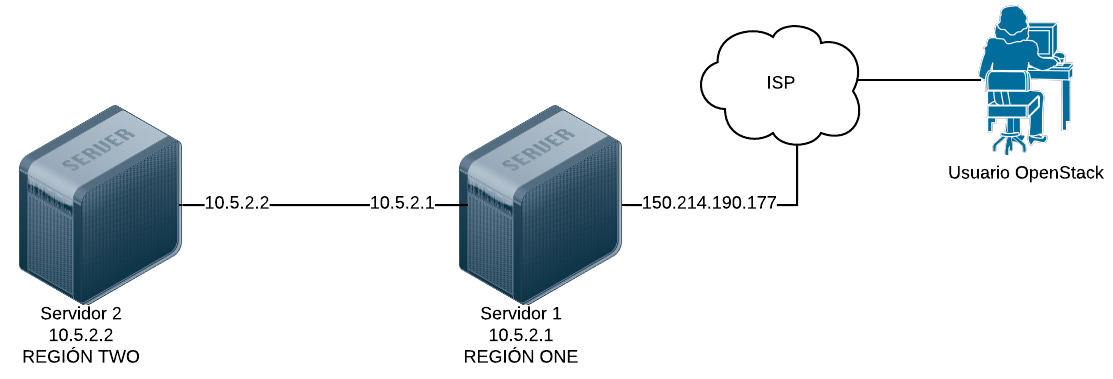
\includegraphics[width=0.7\textwidth]{imagenes/capitulo5/fisico.png}
    \caption{Diseño físico de la infraestructura.}
	\vspace{0.3cm}
    \label{fisico}
\end{figure}

\section{Diseño de un entorno multi-región}

El objetivo de este diseño multi-región, es el de poder usar de forma activa más de una localización geográfica en nuestra cloud proporcionando redundancia, orquestación  y alta disponibilidad, de forma que conseguimos una administración centralizada de nuestra nube, pudiendo disponer de la recuperación de los servicios que se quisieran implementar en la nube ante posibles desastres. 

Si nos fijamos en la Fig.\ref{fisico}, veremos que la Región One, será la implementación de OpenStack con todos sus servicios en el Servidor 1, mientras que la Región Two, será la implementación de OpenStack con todos los servicios que instalemos salvo Keystone y Horizon, pues estos servicios se gestionarán desde el Servidor 1.

Los componentes de la arquitectura por tanto son:

\begin{itemize}
\item Dos implementaciones separadas de OpenStack en la nube, que a su vez equivalen a dos regiones. En este ejemplo, tenemos la Región One y la Región Two \ref{active-active-region}. Estas regiones ejecutan los servicios principales de OpenStack, excepto Keystone y Horizon. Cada región puede tener todos los AZ nodos complementarios que se deseen, aunque en nuestro caso se pondrá un único nodo en cada una.
\item Otra región OpenStack dedicada exclusivamente a hospedar los servicios Keystone y Horizon. Esta región podría clasificarse como la región de administración. En el despliegue que haremos, debido a que sólo disponemos de dos servidores, los servicios de Keystone y Horizon se desplegarán en uno de los servidores, el Servidor 1, que equivale en la Fig.\ref{active-active-region} a la Región One.
\item Las regiones One y Two aprovechan la región de administración para gestionar la autenticación y la interfaz web de la GUI al centralizar la gestión y creación de usuarios, inquilinos y proyectos, proporcionando un solo dashboard para administrar todas las regiones activas.
\end{itemize}


Debida a las limitaciones presentadas, en la sección \ref{subsec:DespliegueProduccion}, se propone el despliegue de un entorno en producción donde se pueda disponer de más nodos.

\begin{figure}
    \centering
    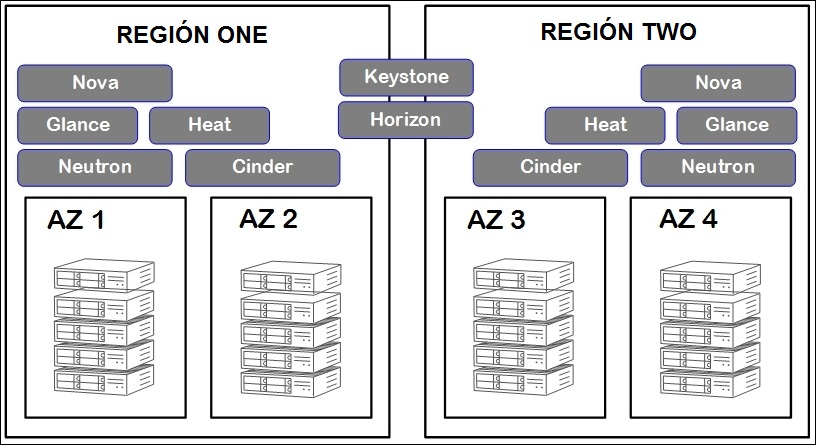
\includegraphics[width=0.7\textwidth]{imagenes/capitulo5/active-active-region.png}
    \caption{Entorno Multi-Región.}
	\vspace{0.3cm}
    \footnotesize{Fuente: Walter Bentley, "OpenStack Administration with Ansible 2 - Second Edition" Packt Publishing, 2016 }
    \label{active-active-region}
\end{figure}

\section{Diseño lógico}
Una vez hayamos conseguido implementar esta configuración los objetivos de diseño serán varios, resultando el esquema de la Fig.\ref{logicoSDN}:

\begin{figure}
    \centering
    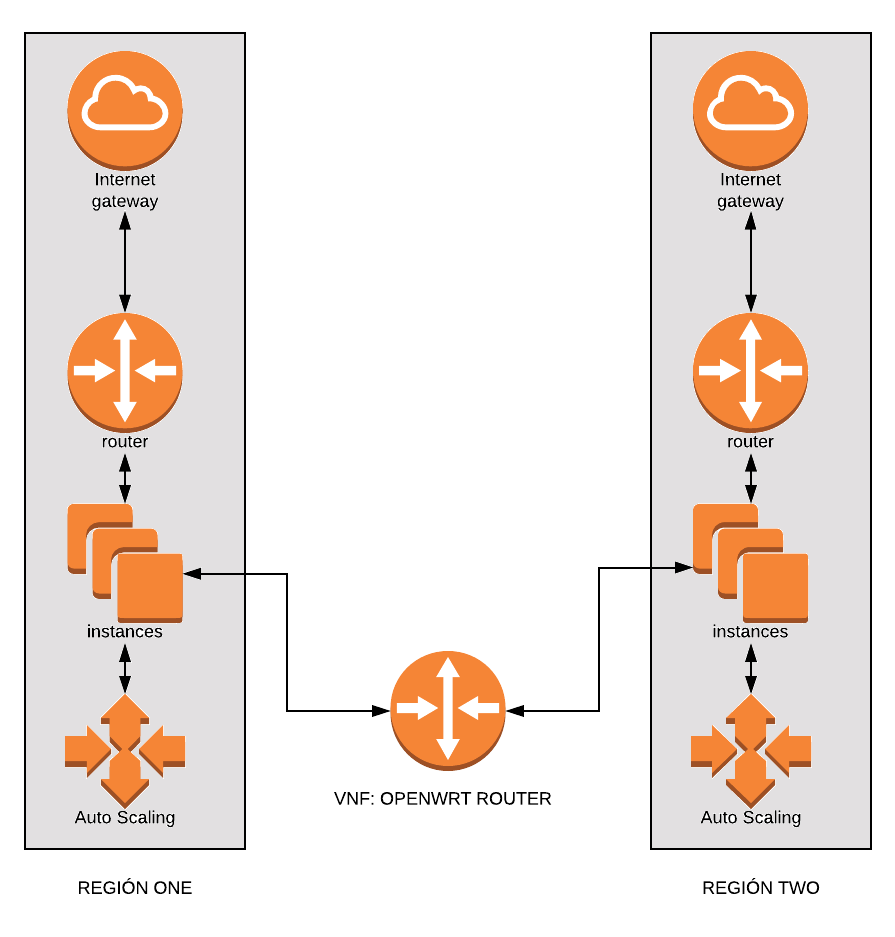
\includegraphics[width=0.7\textwidth]{imagenes/capitulo5/logico.png}
    \caption{Diseño del escenario de red a crear con OpenStack.}
	\vspace{0.3cm}
    \label{logicoSDN}
\end{figure}

\begin{tcolorbox}[colback=red!5!white,colframe=red!75!black]
En este esquema se puede poner también floating IP, y diferenciar entre las distintas capas y la red interna y externa.
\end{tcolorbox}

\begin{itemize}
\item Configurar un esquema de red SDN, basado en un esquema de red jerárquico por capas conforme a lo aprendido durante el Grado en la especialidad de Telemática. En el tendremos la capa de acceso, donde implementaremos las instancia, y la capa de distribución con core colapsado que estará formada por los routers SDN que nos darán acceso a la red externa.
\item Este esquema de red se creará en primer lugar en la Región One, a través del dashboard de Horizon.
\item En la Región Two, implementaremos un esquema de red similar pero esta vez gestionado desde la CLI.
\item Usaremos Heat para la orquestación de distintas instancias de forma automática en base al uso de la CPU de las mismas. De este modo estaremos haciendo gestión de NFVs y autoescalado con el uso de HOT.
\item Por último, crearemos una VNF que en este caso será un router OpenWRT, para interconectar instancias de ambas regiones con el uso de Tacker, realizando así la orquestación de esta NFV en concreto.
\end{itemize}

\subsection{Requisitos del diseño lógico}
Para llevar a cabo este diseño, necesitaremos crear algunos recursos:

\begin{itemize}
\item Creación del entorno SDN. Se crearán los routers, redes y subredes necesarios para la implementación de los escenarios tal y como se verá en el siguiente capítulo.
\item Floating IP. Lo ideal para crear IPs flotantes sería disponer de varias IPs públicas, dado que no es el caso, en ambos servidores se crearán interfaces virtuales en las tarjetas de red para poder abordar el problema de disponer de una sola IP pública. El concepto de  IP flotante se verá con detalle en la sección \ref{subsec:IP-flotante} del siguiente capítulo.
\item Listas de acceso / Firewall. Debemos de establecer listas de acceso que actuarán de firewall para declarar el tráfico tanto entrante como saliente que deseamos permitir. En Openstack esto se hace a través de los \textit{security groups}. Crearemos reglas par permitir cualquier tráfico saliente y sólo el tráfico IP, SSH, y HTTP entrante.
\item Instancias. Las instancias se preparan para ser capaces de alojar cualquier servicio que quisiéramos dar.
\item Key Pair. También necesitaremos crear un par de claves público-privadas para acceder a las instancias de forma segura.
\item Imágenes. La forma más sencilla de obtener una imagen de una máquina virtual que funcione con OpenStack es descargar una ya creada. En este caso será Cirros como veremos más adelante, debido a su pequeño tamaño.
\item Almacenamiento. Por defecto, las instancias que creemos no tendrán espacio para el almacenamiento. Con el servicio de Cinder conseguiremos proveer de almacenamiento persistente a las imágenes.
\item HOT. Plantilla de Heat donde definiremos los parámetros necesarios para la orquestación de NFVs de forma que consigamos crear o borrar instancias en función del uso de la CPU de las mismas.
\item TOSCA Template. Plantilla que contendrá el código necesario para crear una VNF que implemente un router OpenWRT que permita interconectar ambas regiones mediante NFV.
\end{itemize}








